\documentclass[11pt]{article}
\usepackage[margin=1in]{geometry}
\usepackage{amsmath,amssymb,graphicx,booktabs,longtable,hyperref,natbib}
\title{Lost or Inaccessible? A Comparative Causal Study of Neuron and Circuit Ablation for Concept Forgetting in Neural Networks}
\author{Author information pending}
\date{Research protocol and implementation draft: October 2026}
\begin{document}
\maketitle
\begin{abstract}
Classification failure after an intervention does not establish that a representation no longer contains class information. We specify a controlled study of neuron and connection ablation in a small multilayer perceptron trained on the cat and dog subset of CIFAR-10. The protocol separates functional degradation, post-intervention decodability, and restoration of the original computation. It combines class-conditioned selectivity, streaming gradient-times-edge attribution, direct interventions, linear and nonlinear probes, and paired statistical comparisons across independently trained models. This document is a research protocol with an implemented software pipeline. Full five-seed experiments have not been executed; no empirical conclusion about information erasure is asserted.
\end{abstract}
\section{Introduction}
A classifier can fail because a useful representation has changed, because its readout is disconnected, or because the intervention has shifted internal activation distributions. These possibilities motivate a causal comparison with explicit recovery measurements. We study a deliberately constrained visual binary task using a fully connected network. Our objective is operational: determine which probe families can decode class labels after particular interventions, and whether restoring original computations recovers behavior. We make no novelty claim pending a broader systematic literature review.
\section{Related Work}
Distributed representation theory emphasizes information carried by patterns over units \citep{hinton1986}. Network Dissection associates individual units with semantic concepts \citep{bau2017}; association does not alone establish causal necessity. Mechanistic studies identify computational subgraphs and validate them using interventions \citep{wang2022,conmy2023}. Causal tracing motivates same-input activation restoration \citep{meng2022}. Probing measures accessibility to a chosen decoder and has substantial interpretive limitations \citep{belinkov2022}. Machine unlearning addresses deletion of training-data influence \citep{cao2015}; zeroing neurons in a frozen classifier is not a certified unlearning method. Transformer studies inform methodology here, but our primary model remains an MLP.
\section{Research Questions and Hypotheses}
H1: Selective units contribute causally, but selectivity need not predict intervention importance. H2: Edge and neuron interventions produce different degradation patterns. H3: A modified classifier may fail while post-intervention representations remain decodable. H4: Selective restoration may recover original behavior without retraining. H5: Recoverability depends on location, budget, and redundancy. Each statement is a hypothesis; null and contrary results must be reported.
\section{Methodology}
\subsection{Model and estimands}
For $a_0=x$, $z_l=W_la_{l-1}+b_l$, and $a_l=\max(0,z_l)$ at hidden layers, let $f(x)$ be the two logits. Define $m_t(x)=f_t(x)-f_{1-t}(x)$. Report overall and balanced accuracy, class recall, macro precision and F1, cross entropy, ROC-AUC, prediction flips, and class-conditioned margins. A binary prediction collapse is not abstention and does not demonstrate erasure.
\subsection{Selectivity and attribution}
For unit $j$, $S_j=\mathbb E[a_j\mid y=0]-\mathbb E[a_j\mid y=1]$. We also measure pooled standardized difference, variance, sparsity, signed dog-label ROC-AUC, direction-free AUC, and $|a_j\partial m_0/\partial a_j|$. Edge contribution is $c_{ji}=W_{ji}a_i$. Signed edge score is $\mathbb E[(\partial m_0/\partial z_j)c_{ji}]$; absolute score averages the absolute product before aggregation. Class-conditioned versions use only examples from the indicated analysis class. For a minibatch, matrix products $W\odot(G^TA)$ and $|W|\odot(|G|^T|A|)$ avoid storing per-example edge tensors.
\subsection{Interventions and candidate circuits}
Neuron interventions replace selected post-ReLU activations by zero. Edge interventions replace effective weights by $W\odot M$, keeping checkpoint weights unchanged. Controls include uniformly sampled, low-ranked, and activation- or weight-magnitude-quantile-matched masks. Repeated controls are nested within training seed. Candidate edge sets are top-ranked supports or unions of complete high-scoring paths found by dynamic programming. We explicitly report weak components and input-to-output reachable edges. A ranked support may be disconnected; attribution is not causal validation. Biases remain intact even in retained-edge computations.
\subsection{Faithfulness and completeness}
For candidate $C$, let $f_C$ retain only its edges and $f_{\setminus C}$ remove its edges. On analysis examples define $D_t=\max(\mathbb E|m_t(f)|,10^{-8})$. We use
\begin{align}
F_t(C)&=1-\mathbb E|m_t(f_C)-m_t(f)|/D_t,\\
K_t(C)&=\mathbb E|m_t(f_{\setminus C})-m_t(f)|/D_t.
\end{align}
These are descriptive normalized intervention measures. Faithfulness can be negative; completeness can exceed one. They are not universal circuit-identification criteria. Retention and removal answer different questions. Candidate interventions are evaluated directly, and test-set edge-ablation outcomes are reported separately.
\subsection{Comparability}
Neuron counts and edge counts are not matched units. We report the fraction of suppressed outgoing connections, affected absolute weight magnitude, intervention location, and $\|A'-A\|_F/\max(\|A\|_F,10^{-12})$. Neuron zeroing suppresses outgoing contributions; its incoming computations still occur. Descriptive performance matching pairs conditions on validation balanced accuracy and reports the matching gap before showing test outcomes.
\subsection{Recoverability and restoration}
Each condition receives an independently fitted linear logistic probe and a 64-unit nonlinear probe. Probe inputs are post-intervention hidden states at the affected layer and subsequent layers. Feature standardization uses probe-training examples only. Probe early stopping uses probe validation loss. Readout-only interventions leave all hidden states unaffected; their final-hidden probes are explicitly labeled pre-readout references. Clean-representation probes provide capacity-matched reference measurements. Better probe performance establishes decodability by that family, not preservation of all original information. Failed probes do not establish erasure. Same-input clean activation patching and selective edge restoration reinstate computations; fitting probes instead trains new readouts. These operations are not equivalent to relearning the original classifier.
\section{Experimental Setup}
Official CIFAR-10 training examples for classes 3 and 5 are remapped to labels 0 and 1 and split into stratified partitions of 8,000 training, 1,000 validation, and 1,000 analysis examples. The official 2,000 test examples are reserved for final outcomes. Channel moments use only the 8,000 model-training images. Probe training and validation use disjoint 6,400/1,600 subsets of model training data; neither uses test examples. These examples were seen by the base model, a limitation distinct from probe-fit leakage. Saved manifests record official example indices and label fingerprints.
The MLP is $3072\to512\to256\to128\to2$ with ReLU, without dropout or normalization layers. AdamW uses learning rate $10^{-3}$, weight decay $10^{-2}$, batches of 128 (64 in the Mac profile), at most 50 epochs, patience 8, and gradient clipping 1. Checkpoints minimize validation loss. Seeds are 42, 123, 456, 789, and 2026. Neuron budgets are 1, 5, 10, 20, and 40 percent. Edge budgets are 0.1, 0.5, 1, 2, 5, and 10 percent globally and per layer. Five random repetitions are used in the full profile. The Mac profile uses one seed, fewer budgets, two repetitions, four circuit-discovery minibatches, and linear probes first. It is a pilot rather than full five-seed evidence.
\subsection{Statistics}
Independent model-training seeds are the replication unit. Random-mask repetitions are averaged within each seed. Report mean, sample standard deviation, and Student-$t$ 95\% intervals, which are unavailable for one seed. Targeted and random controls are paired by model, target, layer, and budget. Report paired effects, Cohen's $d_z$ when defined, and Holm-adjusted paired-test $p$ values. Stratified paired image bootstraps quantify within-model prediction uncertainty separately. They do not replace seed-level inference. Raw edge Jaccard is a descriptive instability diagnostic; neuron permutation prevents interpreting it as semantic circuit equivalence.
\section{Results}
\textbf{TODO: Full research experiments not run.} The repository execution report records software tests separately from CIFAR-10 experiments. No hypothesis is accepted or rejected here. Figure~\ref{fig:design} describes the protocol; measured figures are included only when exported from executed runs. Tables~\ref{tab:setup} and \ref{tab:baseline} distinguish configured setup from observed results.
\begin{figure}[ht]\centering
\IfFileExists{figures/F1_architecture.pdf}{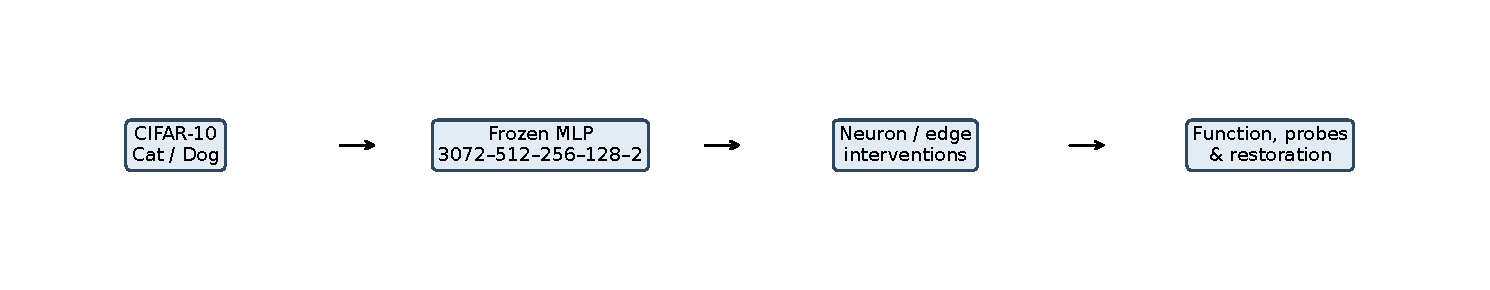
\includegraphics[width=\linewidth]{figures/F1_architecture.pdf}}{\fbox{CIFAR-10 $\to$ MLP $\to$ interventions $\to$ recovery evaluation}}
\caption{Research protocol; this diagram contains no experimental observations.}\label{fig:design}\end{figure}
\begin{table}[ht]\centering\begin{tabular}{ll}\toprule Item&Configuration\\\midrule Hidden units&512, 256, 128\\ Activation&ReLU\\ Optimizer&AdamW\\ Selection&Validation loss\\\bottomrule\end{tabular}\caption{Primary setup.}\label{tab:setup}\end{table}
\begin{table}[ht]\centering\begin{tabular}{ll}\toprule Experiment&Status\\\midrule Five-seed baseline&Not run\\ Full intervention study&Not run\\ Full recovery study&Not run\\\bottomrule\end{tabular}\caption{Research results pending execution; see the execution report for pilot status.}\label{tab:baseline}\end{table}
\subsection{Planned empirical reporting}
TODO: Discuss measured learning curves (F2), selectivity (F3), neuron ablation (F4), connectivity and attribution (F5), edge interventions (F6), comparison (F7), probes (F8--F10), restoration (F11), and seed robustness (F12). Exported tables T1--T10 contain setup, baseline, selectivity, ablations, circuits, comparisons, probes, restoration, and statistics. Missing observations must remain marked not run. Do not use software smoke-test figures as research figures.
\section{Discussion}
A gap between an original readout and a new probe would indicate readout-relative inaccessibility under the tested conditions. Such a gap would not by itself establish that the same representation or mechanism survived intact. Restoration of behavior would show sufficiency of restored components in context, rather than uniqueness or minimality of a circuit. These are conditional interpretations for future measurements, not findings from this draft.
\section{Limitations}
Binary cat/dog classification lacks abstention and can hide asymmetric class collapse. An MLP over flattened pixels has restricted visual inductive bias. Zero interventions can generate out-of-distribution hidden states. Gradient scores are local and may miss nonlinear interactions. Magnitude-bin matching is approximate and can overlap selected supports. Fixed probe families cannot establish information-theoretic absence. Probe datasets overlap base-model training data, although probe evaluation is held out. Five seeds provide limited statistical power, while a one-seed pilot supports no model-population inference. Hardware-level nondeterminism and unaligned hidden units limit cross-device and cross-seed equivalence claims. No certified unlearning or privacy claim is made.
\section{Conclusion}
We provide an executable protocol for separating functional loss, decoder-relative recoverability, and computational restoration in a small MLP. Full experiments remain necessary before drawing conclusions about the five hypotheses or class information loss.
\bibliographystyle{plainnat}\bibliography{references}
\appendix
\section{Reproducibility and Artifact Audit}
Run configurations and source fingerprints identify output directories. Split manifests, checkpoints, intervention masks, predictions, probe parameters, environment logs, and per-condition completion markers support audit and resume. Failed stages retain diagnostics. CPU is the portable fallback; CUDA and MPS require local verification. See README.md and docs/METHODOLOGY.md for commands, operational definitions, and troubleshooting.
\section{Generated Tables}
Generated long tables can be copied from a completed run into paper/tables using the export script. Each export records the source run. The manuscript must be updated only after inspecting the execution status and corresponding measured outputs.
\end{document}
